\documentclass[linenumbers]{aastex702}

\newcommand{\asgard}{\textsc{ASGARD}}
\newcommand{\grb}{gamma-ray burst}
\newcommand{\grbs}{gamma-ray bursts}
\newcommand{\eats}{equal-arrival-time surface}
\newcommand{\fshock}{forward shock}
\newcommand{\rshock}{reverse shock}
\newcommand{\fnu}{F_\nu}

\shorttitle{ASGARD GRB Afterglow Toolkit}
\shortauthors{Ren}

\begin{document}

\title{\asgard: A Radius-Resolved Toolkit for Gamma-Ray Burst Afterglow Radiation, Hadronic Feedback, and Observer Projection}

\author[0000-0000-0000-0000]{Jia Ren}
\affiliation{Affiliation to be supplied}
\email{email to be supplied}

\begin{abstract}
Interpreting multiwavelength \grb\ afterglows requires a calculation that keeps blast-wave dynamics, particle transport, local photon fields, absorption, and observer projection in the same physical bookkeeping system.  Many public workflows provide efficient synchrotron light curves for structured jets, but fewer expose the intermediate electron, hadron, photon-field, and reverse-shock states needed to test feedback-dominated scenarios or to diagnose numerical failures.  We present \asgard, a Python and Fortran toolkit for \grb\ afterglow modeling and fitting.  The public interface constructs a physical model from jet, external-medium, radiation, numerical, observer, reverse-shock, and hadronic options, while the compiled kernels advance the radius-ordered dynamics, electron transport, synchrotron and synchrotron self-Compton emission, gamma-gamma absorption, one-dimensional hadronic transport, reverse-shock emission, polarization, and observer-frame projection.  The code stores the local state on the shock-radius grid and applies observer time only at the final projection stage, which prevents post-processing fixes from replacing local conservation or source-sink accounting.  We describe the API, numerical contracts, validation artifacts, and explicitly unsupported backend boundaries.  Reproducible figures generated from the repository demonstrate public light-curve and spectrum queries, one- and two-dimensional electron transport timing, shell-level hadronic feedback roles, magnetized reverse-shock diagnostics, secondary reverse-shock energy accounting, and runtime composition.  The present release is a code and methods baseline rather than a single-event fit; its formal hadronic path is one-dimensional, and chi-resolved hadronic feedback and inverse-Compton-mediated electromagnetic cascades remain outside the implemented contract.
\end{abstract}

\keywords{Gamma-ray bursts (629) --- Computational methods (1965) --- Astronomy software (1855) --- Radiative processes (2055) --- Non-thermal radiation sources (1119)}

\section{Introduction} \label{sec:intro}

Gamma-ray burst afterglows are produced when relativistic ejecta transfer energy to the circumburst medium and accelerate nonthermal particles.  The standard synchrotron framework links the blast-wave dynamics, electron distribution, spectral breaks, and observer-frame light curves \citep{Sari1998,Granot2002}.  Modern afterglow work also requires structured jets, off-axis viewing, inverse-Compton channels, reverse shocks, polarization, and in some cases hadronic emission or secondary-pair feedback.  These additions make the problem more than a mapping from parameters to a flux density: the calculation must track where each particle and photon source term lives, which coordinate it uses, and which quantities are projected to the observer only after local evolution has been solved.

Open-source astrophysical software has become central to reproducible inference.  Packages such as \texttt{afterglowpy}, \texttt{Astropy}, \texttt{Gammapy}, \texttt{MOSFiT}, and \texttt{naima} show that a code paper is most useful when it documents not only an interface, but also the physical assumptions, data products, validation paths, and limits of the implementation \citep{Ryan2020,Ryan2024,Astropy2022,Gammapy2023,Guillochon2018,Zabalza2015}.  For \grb\ afterglows, the public afterglow ecosystem already includes efficient structured-jet synchrotron models and hydrodynamic-calibrated light-curve prescriptions \citep{vanEerten2010,Ryan2020}.  The complementary need addressed here is a radius-resolved research toolkit in which intermediate electron, hadron, photon-field, reverse-shock, and observer states remain inspectable and tied to explicit numerical contracts.

\asgard\ is designed around that requirement.  The code uses Python for public model construction, orchestration, fitting, and data products, and Fortran for the high-cost dynamics, transport, radiation, and projection kernels.  Its central state is ordered by shock radius rather than by observer time.  Observer time enters through an \eats\ projection after local particle and photon evolution has been assembled.  This separation is important for feedback problems: Bethe-Heitler pair production, pair-synchrotron cascades, photopion photon survival, and inverse-Compton cooling must be converted to the same shell coordinate before they can be compared or coupled.

This paper documents the current code and methods baseline.  Section~\ref{sec:design} gives the software architecture and public interface.  Section~\ref{sec:physics} describes the implemented physical modules.  Section~\ref{sec:numerics} records the numerical contracts that define the kernels and state objects.  Section~\ref{sec:verification} presents reproducible figure-level validation artifacts.  Section~\ref{sec:limits} states the boundaries that are intentionally not implemented in this release.

\section{Software Design and Public Interface} \label{sec:design}

\subsection{Radius-first state model}

The one-sentence argument of this manuscript is: in \grb\ afterglow modeling, \asgard\ shows that a radius-ordered state chain can keep electron, hadron, photon, reverse-shock, and observer products in one reproducible calculation, supported by public API smoke tests, build checks, benchmark artifacts, and source-data-backed figures, with the boundary that formal hadronic feedback is currently one-dimensional.

Figure~\ref{fig:architecture} summarizes the design.  A user constructs a \texttt{Model} from public dataclasses for the jet, medium, observer, radiation, numerical grid, solver options, reverse shock, and hadronic options.  These objects are normalized to a \texttt{RuntimeConfig} and a \texttt{SimulationSetup}.  A solve then produces a \texttt{SolveState} containing dynamics, electron, photon-field, hadronic, reverse-shock, observer, and component objects.  Downstream products such as light curves, spectra, sky images, polarization curves, and fitting likelihoods are derived from that state.

\begin{figure}[!tp]
  \centering
  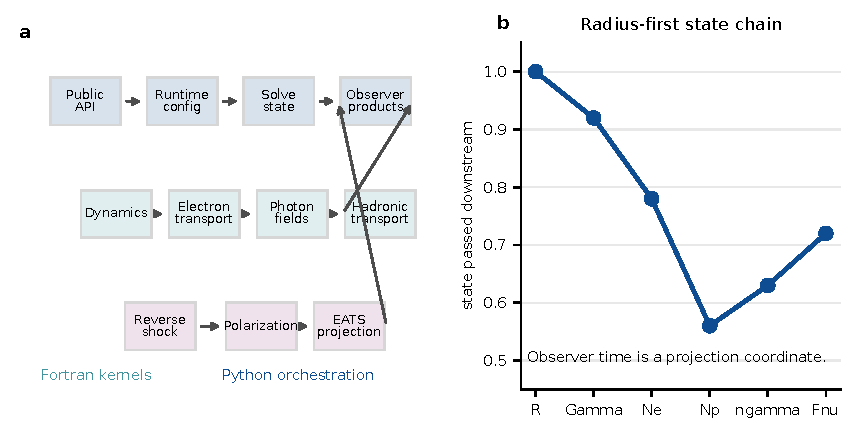
\includegraphics[width=\textwidth]{figures/fig1_architecture.pdf}
  \caption{Architecture and coordinate contract of \asgard.  (a) Public Python objects are normalized into runtime state, while the expensive dynamics, particle-transport, radiation, and projection stages are handled by compiled kernels.  (b) The main state chain is ordered by shock radius; observer time is introduced at the projection stage rather than used as the shared coordinate for local feedback.  Source data are in \texttt{source\_data/fig1\_architecture\_nodes.csv} and \texttt{source\_data/fig1\_architecture\_edges.csv}.}
  \label{fig:architecture}
\end{figure}

The public query methods are \texttt{flux\_density\_grid}, \texttt{flux\_density}, \texttt{spectrum}, \texttt{flux}, \texttt{sky\_image}, \texttt{polarization}, and \texttt{details}.  The fitting interface uses the same state construction and projection path, so likelihood evaluation and standalone model queries are not separate physical implementations.  \asgard\ also records component-level fluxes, including forward-shock synchrotron and synchrotron self-Compton (SSC), reverse-shock synchrotron and SSC, cross-zone inverse-Compton terms when enabled, and hadronic components.

\subsection{Terminology ledger}

The manuscript uses the following canonical terms.  \emph{Forward shock} refers to the blast wave propagating into the external medium.  \emph{Reverse shock} refers to the shocked ejecta region and its region-3 thermal state.  \emph{Shell-level} means a quantity is stored on the radius grid without resolving the downstream chi coordinate.  \emph{Chi-resolved} means that the electron distribution or projection uses the finite-thickness downstream coordinate \(\chi\).  \emph{Joint feedback} means the opt-in shell-level coupling of electrons, photon fields, formal hadronic transport, and secondary pairs.  \emph{Observer projection} means the \eats\ and Doppler mapping from local luminosity to \(\fnu(t_{\rm obs})\).

\section{Physical Modules} \label{sec:physics}

The implemented physical chain is
\[
{\rm ejecta}
\rightarrow {\rm shocks}
\rightarrow N_e,\ N_p,\ n_\gamma
\rightarrow L_\nu'
\rightarrow F_\nu(t_{\rm obs}).
\]
The forward shock supplies \(R_i\), \(\Gamma_i\), swept-up mass, external density, and observer-time mapping.  The default external media are a uniform interstellar medium and a \(k=2\) wind.  Density jumps and injection events are represented as explicit model inputs; if a smooth physical configuration produces an isolated discontinuity in spectra, light curves, or characteristic quantities, the code treats that as a numerical or physical bug rather than as a feature to hide by smoothing.

Electrons are advanced on a logarithmic Lorentz-factor grid.  The one-dimensional solvers include \texttt{fullhide\_1d}, \texttt{slc1\_1d}, \texttt{charint\_1d}, \texttt{t2g1\_1d}, and \texttt{weno5\_1d}.  The two-dimensional solvers \texttt{fullhide\_2d} and \texttt{charint\_2d} add a downstream finite-thickness coordinate.  The default stable public path is \texttt{fullhide\_1d}; two-dimensional transport and chi-resolved projection are opt-in paths used when the finite shell width is part of the hypothesis being tested.

The photon field is represented separately from observer luminosity.  This distinction is required because an observer-side luminosity is not automatically a local target photon density.  SSC cooling and emission, gamma-gamma absorption, photopion targets, Bethe-Heitler photon losses, and pair-synchrotron feedback require explicit shell geometry, escape-time, and unit conversions before they can be coupled.

The formal hadronic path uses a one-dimensional shell contract.  Proton transport, proton synchrotron, photopion interactions, Bethe-Heitler pair production, \(pp\) processes, secondary species transport, secondary radiation, gamma-gamma pair production, pair-synchrotron cascades, hadronic inverse-Compton emission, and neutrino output are exposed through runtime options when the formal solver is selected.  The photopion operator follows the response-function approach of \citet{Hummer2010}.  In joint feedback mode, only secondary electron spectra and photon sink/source terms that are explicitly output by the formal kernels enter the electron and photon equations.

The reverse-shock baseline includes electron synchrotron radiation, reverse-shock SSC, forward/reverse cross-zone IC, optional upstream magnetization, and optional reverse-shock hadronic branches.  The reverse-shock electron injection scale is tied to the shock-front \(\gamma_{34}\).  The turbulent magnetic field uses the region-3 thermal state \(U_3/V_3\), and optional upstream magnetization adds an ordered component to the total \(B_3\).  The \(\sigma \rightarrow 0\) limit is a validation boundary: it must recover the unmagnetized baseline.

\section{Numerical Contracts} \label{sec:numerics}

\subsection{Radius coordinate and rate conversion}

The local evolution coordinate is shock radius \(R\).  For a shell with Lorentz factor \(\Gamma\) and velocity \(\beta c\),
\[
  \frac{dt'}{dR} = \frac{1}{\beta \Gamma c}.
\]
Any comoving rate in units of \({\rm s}^{-1}\) must be converted through this factor before entering a radius-coordinate transport equation.  This rule applies to electron cooling, proton losses, secondary injection, and photon absorption.  It is also the reason joint electron-photon-hadron feedback is not implemented as an observer-time post-processing correction.

\subsection{Particle and photon grids}

Electron and proton spectra use logarithmic grids.  If \(x=\log_{10}\gamma\), the transported cell content is \(dN/dx\), not \(dN/d\gamma\).  Conversions therefore carry the Jacobian
\[
  \frac{dN}{d\gamma} =
  \frac{1}{\gamma \ln 10} \frac{dN}{dx}.
\]
The same bookkeeping applies to frequency grids: \(L_\nu d\nu = \widetilde{L}_{\ln\nu} d\ln\nu\).  The implementation keeps these conversions at the kernel boundaries and in state assembly, so that observer projection receives luminosities with the expected units.

\subsection{Observer projection}

The observer stage maps local comoving luminosities to \(\fnu(t_{\rm obs})\) using Doppler factors, redshift, luminosity distance, and \eats\ interpolation.  The chi-resolved kernel applies only to forward-shock synchrotron plus synchrotron self-absorption in the current release.  SSC, hadronic components, and pair cascades remain shell-level contributions unless a future physical contract defines their chi-local photon fields, particle densities, feedback, and projection.

\section{Verification and Demonstrations} \label{sec:verification}

The repository is tested through build gates, line-truncation checks, smoke tests, and benchmark artifacts.  For the baseline used in this manuscript, the electron fullhide, electron charint-2D, and reverse-shock extensions were rebuilt; the README public-query smoke test, fullhide-2D smoke benchmark, reverse-shock smoke test, and line-truncation source-closure check passed.  Figure source data are generated by \texttt{tests/generate\_paper\_figures.py}.

\begin{figure}[!tp]
  \centering
  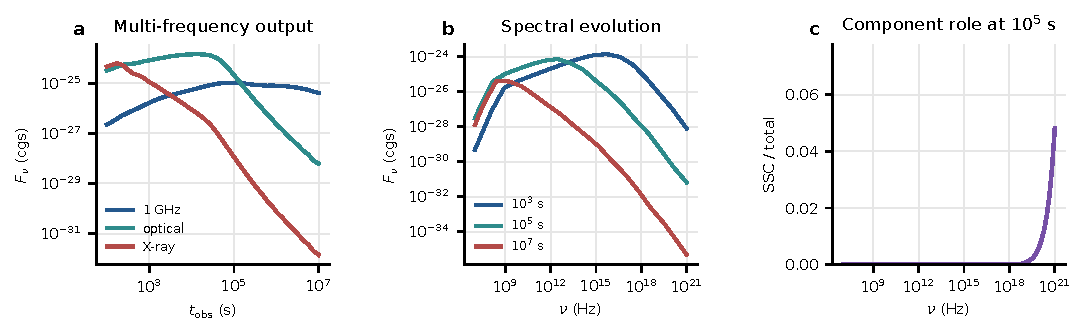
\includegraphics[width=\textwidth]{figures/fig2_forward_api.pdf}
  \caption{Public forward-shock API demonstration.  (a) A single \texttt{Model} query returns multi-frequency light curves.  (b) The same model returns a broadband spectrum at fixed observer time.  (c) Component accounting keeps synchrotron and SSC terms separate before they are summed into the total flux.  Source data are in \texttt{source\_data/fig2\_forward\_api.csv}.}
  \label{fig:forwardapi}
\end{figure}

Figure~\ref{fig:forwardapi} shows a public API calculation for a top-hat forward-shock model.  The figure is not intended as a fit to a particular burst; it demonstrates that the same state chain returns light curves, spectra, and component-resolved fluxes through the public interface.  The source data record the input observer times, frequencies, total fluxes, forward-shock synchrotron fluxes, and SSC fluxes.

\begin{figure}[!tp]
  \centering
  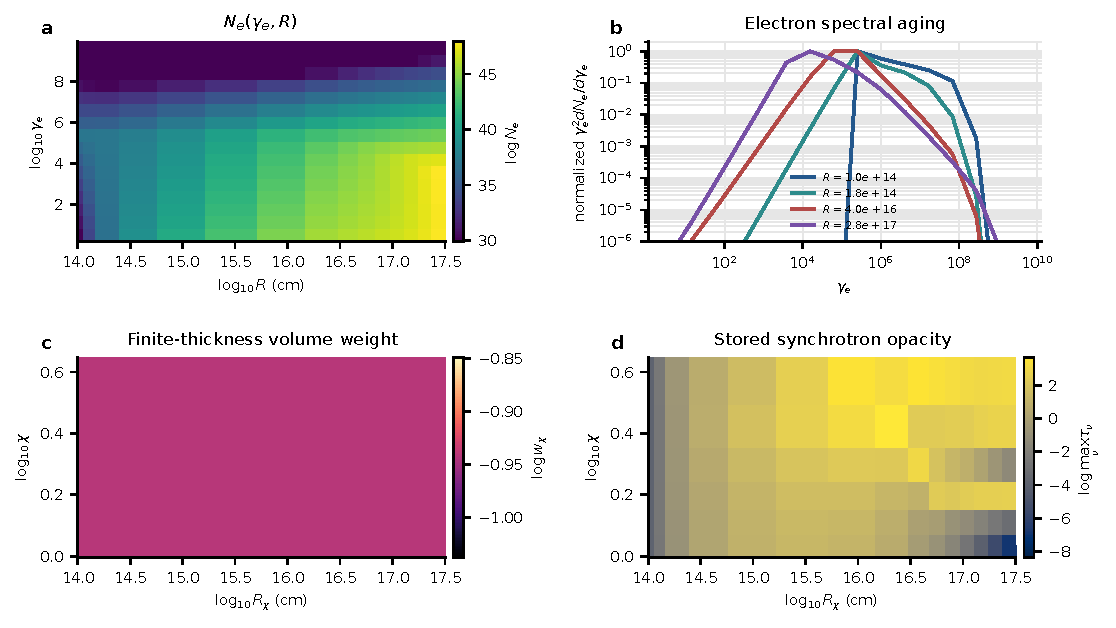
\includegraphics[width=\textwidth]{figures/fig3_transport_projection.pdf}
  \caption{Electron transport and projection contracts.  (a) One-dimensional and chi-resolved electron paths differ in the state they pass to the observer projection.  (b) Runtime benchmark summaries compare one- and two-dimensional public solve paths for ISM and wind cases.  (c) A representative two-dimensional profile shows that electron transport dominates the benchmarked cost in this configuration.  Source data are in \texttt{source\_data/fig3\_transport\_projection\_runtime.csv}.}
  \label{fig:transport}
\end{figure}

Figure~\ref{fig:transport} documents both the algorithmic distinction and the cost boundary of chi-resolved transport.  The benchmark is not used to claim universal performance; it fixes a reproducible reference configuration and identifies where runtime is spent.  This is the appropriate use of a methods-paper benchmark: it supports a decision about which solver path is suitable for a given physical question.

\begin{figure}[!tp]
  \centering
  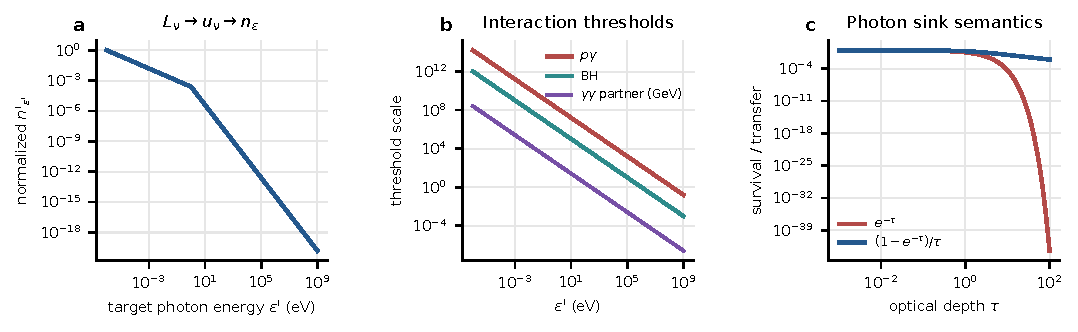
\includegraphics[width=\textwidth]{figures/fig4_hadronic_feedback.pdf}
  \caption{Hadronic and joint-feedback contract.  (a) Shell-level joint feedback couples protons, photons, and secondary pairs only through explicitly modeled source and sink terms.  (b) Implemented process roles distinguish observer luminosity from feedback into the electron equation or photon field.  Source data are in \texttt{source\_data/fig4\_hadronic\_feedback\_contract.csv}.}
  \label{fig:hadronic}
\end{figure}

Figure~\ref{fig:hadronic} states the feedback contract rather than hiding it inside a switch name.  Proton synchrotron and neutrinos are observer outputs.  Bethe-Heitler, \(pp\), and gamma-gamma pair/synch branches can feed secondary pairs when the formal kernel supplies the spectrum and normalization.  Photopion and Bethe-Heitler photon losses act on the photon field only through explicitly calculated survival or loss terms.  The code does not synthesize missing spectra from total energy budgets.

\begin{figure}[!tp]
  \centering
  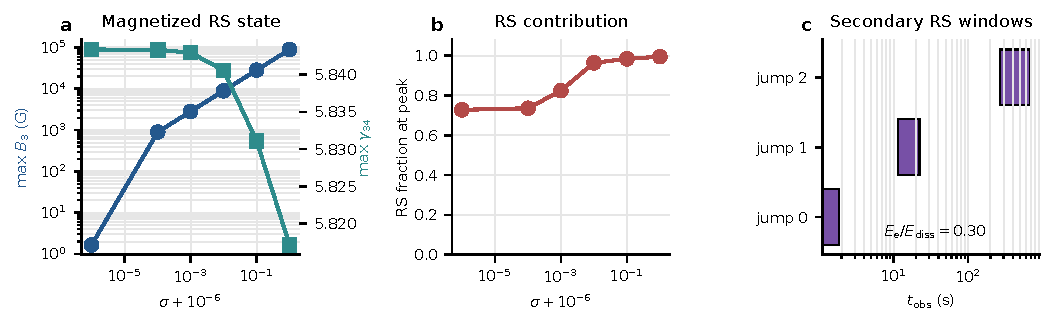
\includegraphics[width=\textwidth]{figures/fig5_reverse_shock.pdf}
  \caption{Reverse-shock diagnostics.  (a) Magnetized reverse-shock scans track the total region-3 magnetic field and \(\gamma_{34}\).  (b) The reverse-shock contribution at the optical peak changes with upstream magnetization in the benchmark configuration.  (c) Density-jump-triggered secondary reverse shocks have explicit observer-time windows and energy accounting.  Source data are in \texttt{source\_data/fig5\_reverse\_shock\_sigma\_summary.csv}, \texttt{source\_data/fig5\_reverse\_shock\_lightcurve\_summary.csv}, \texttt{source\_data/fig5\_secondary\_rs\_events.csv}, and \texttt{source\_data/fig5\_secondary\_rs\_energy.csv}.}
  \label{fig:rs}
\end{figure}

Figure~\ref{fig:rs} shows how reverse-shock diagnostics are recorded.  The magnetized benchmark treats VegasAfterglow as a comparison backend for jump-condition behavior, not as the target truth for \asgard\ light curves.  The secondary reverse-shock summary records the dissipated energy and injected electron energy directly; this prevents density-jump features from being introduced as phenomenological light-curve patches.

\begin{figure}[!tp]
  \centering
  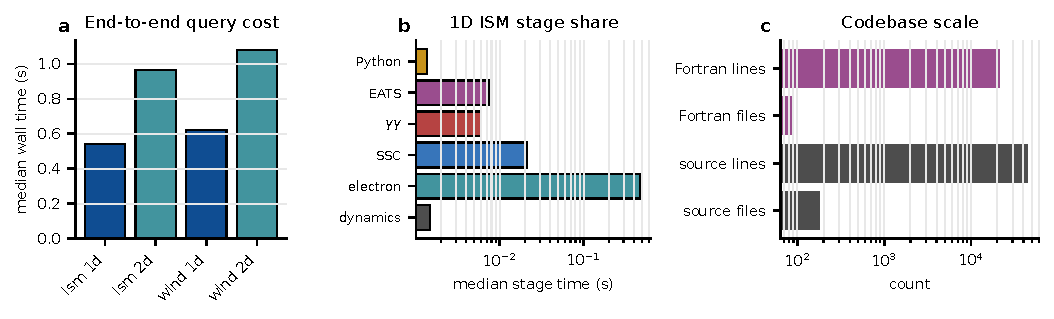
\includegraphics[width=\textwidth]{figures/fig6_runtime_reuse.pdf}
  \caption{Runtime and reuse summary.  (a) End-to-end public query cost for tracked benchmark configurations.  (b) Stage-level decomposition for an ISM one-dimensional run.  (c) Current tracked codebase scale.  Source data are in \texttt{source\_data/fig6\_runtime\_summary.csv} and \texttt{source\_data/fig6\_code\_metrics.csv}.}
  \label{fig:runtime}
\end{figure}

Figure~\ref{fig:runtime} frames performance as a reproducibility diagnostic.  The benchmark records the full command context in the repository documentation and separates high-level query time from low-level stage timing.  The codebase scale panel is included to make clear that the Fortran kernels are a substantial part of the implementation, not an incidental acceleration layer around a Python-only model.

\section{Limitations and Unsupported Boundaries} \label{sec:limits}

Several public options are intentionally bounded.  Jet spreading is not implemented in the current structured/top-hat backend.  User-defined \texttt{Medium} kernel dispatch is not supported; the compiled density contract covers uniform media and \(k=2\) winds.  Wind profiles with \(k \ne 2\) are rejected rather than silently approximated.  Thermal electrons are supported only in the \texttt{fullhide\_1d} branch.  Toroidal polarization is not supported for non-axisymmetric jets.

The formal hadronic path is one-dimensional and shell-level.  A chi-resolved hadronic implementation would require chi-local photon fields, hadron densities, secondary feedback, and observer projection before it could be physically meaningful.  Similarly, the current pair cascade is a gamma-gamma pair/synchrotron branch.  An inverse-Compton-mediated electromagnetic cascade would require additional photon and pair source-sink equations and an energy-budget benchmark.  These omissions are scientific boundaries, not missing fallback code.

The manuscript also does not claim that the validation examples exhaust the physical model space.  They are targeted tests selected because they answer decisions about public query behavior, coordinate contracts, source-sink accounting, reverse-shock diagnostics, and runtime composition.  Low-information sweeps that would only repeat known unsupported cases are deliberately not included.

\section{Summary} \label{sec:summary}

\asgard\ provides a radius-resolved \grb\ afterglow toolkit that exposes public model queries while preserving inspectable intermediate states for dynamics, electrons, photon fields, hadrons, reverse shocks, polarization, and observer projection.  The code design separates Python orchestration from Fortran numerical kernels and keeps local feedback on the shock-radius grid before observer-time projection.  The present paper records the method contracts, source-data-backed figures, validation checks, and explicit backend limits for the current baseline.  This makes \asgard\ a reproducible platform for afterglow modeling work where the numerical path and physical boundary conditions must be auditable, not only a generator of final light curves.

\clearpage
\appendix

\section{Claim-evidence map} \label{app:claims}

\noindent\textbf{Radius-first state chain.}  Evidence: Figure~\ref{fig:architecture}, public code structure in \texttt{asgard\_core}, and documented \texttt{SolveState} objects.  Status: supported.

\noindent\textbf{Component-resolved public queries.}  Evidence: Figure~\ref{fig:forwardapi}, \texttt{FluxResult.total}, \texttt{fwd.sync}, and \texttt{fwd.ssc} source data.  Status: supported.

\noindent\textbf{Chi-resolved electron transport.}  Evidence: Figure~\ref{fig:transport} and the tracked runtime benchmark CSV.  Status: supported for the benchmark configuration, and opt-in relative to the shell-level path.

\noindent\textbf{Hadronic feedback contract.}  Evidence: Figure~\ref{fig:hadronic} and the joint-feedback physics and algorithm documents.  Status: supported only through explicit source-sink outputs.

\noindent\textbf{Reverse-shock diagnostics.}  Evidence: Figure~\ref{fig:rs} and tracked sigma and secondary-RS source data.  Status: supported for the benchmark configuration.

\noindent\textbf{Unsupported future branches.}  Evidence: Section~\ref{sec:limits}, public backend limits, and TODO boundary documents.  Status: chi-resolved hadronic transport and IC-mediated electromagnetic cascades are unsupported boundaries.

\section{Build and verification record} \label{app:build}

The implementation baseline for this manuscript is git commit \texttt{2cf7eaecda0b}.  Before drafting the paper, the following checks were run in WSL Ubuntu through \texttt{rtk}: text encoding check, \texttt{git diff --check}, forced builds of \texttt{electron\_forward\_\allowbreak fullhide\_1d}, \texttt{electron\_forward\_\allowbreak charint\_2d}, and \texttt{electron\_reverse\_\allowbreak kernel}, public README smoke test, fullhide-2D smoke benchmark, reverse-shock smoke test, and a \texttt{gfortran -Werror=line-truncation} source-closure syntax check over the affected electron extensions.  The manuscript itself is compiled with Windows-side TeX Live.

\software{\asgard\ \citep{ASGARDSoftware}, Python, NumPy \citep{Harris2020}, SciPy \citep{Virtanen2020}, Matplotlib \citep{Hunter2007}, Astropy \citep{Astropy2022}, emcee \citep{ForemanMackey2013}, gfortran, f2py}

\begin{acknowledgments}
Acknowledgments, funding information, and final author metadata are to be supplied by the author before submission.  Use of language-model assistance in drafting and code generation should be disclosed according to the current AAS policy if this manuscript is submitted.
\end{acknowledgments}

\bibliographystyle{aasjournalv7.1}
\bibliography{references}

\end{document}
